\chapter{TikZ e plotting}
\section{Boxes}
\begin{verbatim}
\boxed{Prova}
\end{verbatim}
$$\boxed{Prova}$$

\begin{verbatim}
	\RiquadroOmbra{Testo}
\end{verbatim}
\RiquadroOmbra{Testo}

\begin{verbatim}
	\begin{TitoloIntro}[colbacktitle=red]{Titolo}{Testo}\end{TitoloIntro}
\end{verbatim}
\begin{TitoloIntro}[colbacktitle=red, width=\textwidth]{Titolo}{Testo}\end{TitoloIntro}

\begin{verbatim}
	\begin{RTitoloIntro}[colbacktitle=red]{Titolo}{Testo}\end{RTitoloIntro}
\end{verbatim}
\begin{RTitoloIntro}[colbacktitle=red]{Titolo}{Testo}\end{RTitoloIntro}

\begin{verbatim}
	\begin{BoxTitolo}{Titolo}{Testo}\end{BoxTitolo}
\end{verbatim}
\begin{BoxTitolo}{Titolo}{Testo}\end{BoxTitolo}
%%%%%%%%%%%%%%%%%%%%%%%%%%%%%%%%%%%%%%%%%%%%%%%%%%%%%%

\newpage
\section{PGF (per info sul typesetting -> "pgfplots" su ctan.org)}
\index{Esempio}
\begin{center}
\fbox{\parbox{.8\textwidth}{Questa sezione contiene solo alcuni esempi: visto che su Overleaf è stata ridotto il tempo di compilazione ho sostituito il codice in verbatim con uno screenshot dell'immagine risultante compilando tale codice}}
\end{center}
\vspace{2cm}

\begin{verbatim}
	\begin{figure}[ht]\centering
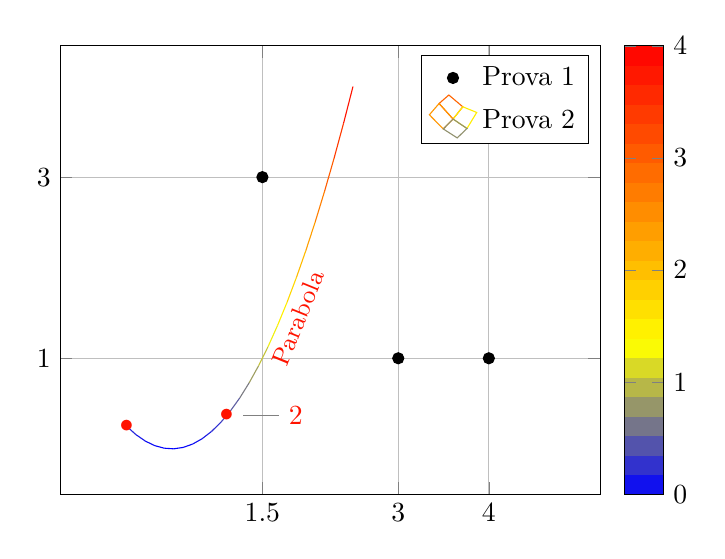
\begin{tikzpicture} \begin{axis}[xmin=-0.5, xmax=5, ymin=-0.5,
	colorbar sampled, colorbar style={samples=24}, 
	axis equal, xtick=data, ytick=data, grid=major]
    \addplot[only marks] coordinates { (4,1) (3,1) (1.5,3) };
   	\addplot[mesh, domain=0:2.5, tick=\empty] {(x-.5)^2}  node [pos=0]  {$\bullet$}      
   	node [pos=0.25, pin=0.4:2 ] {$\bullet$}
   	node [pos=0.5, sloped, xshift=0cm, yshift=-.2cm] {\small Parabola}; 
     \legend{Prova 1, Prova 2};     
\end{axis}	
\end{tikzpicture}\noindent\hspace{2cm}
\caption{Colormap, legenda, punti e grafici di funzione}
    \end{figure}
\end{verbatim}

\begin{figure}[ht]\centering
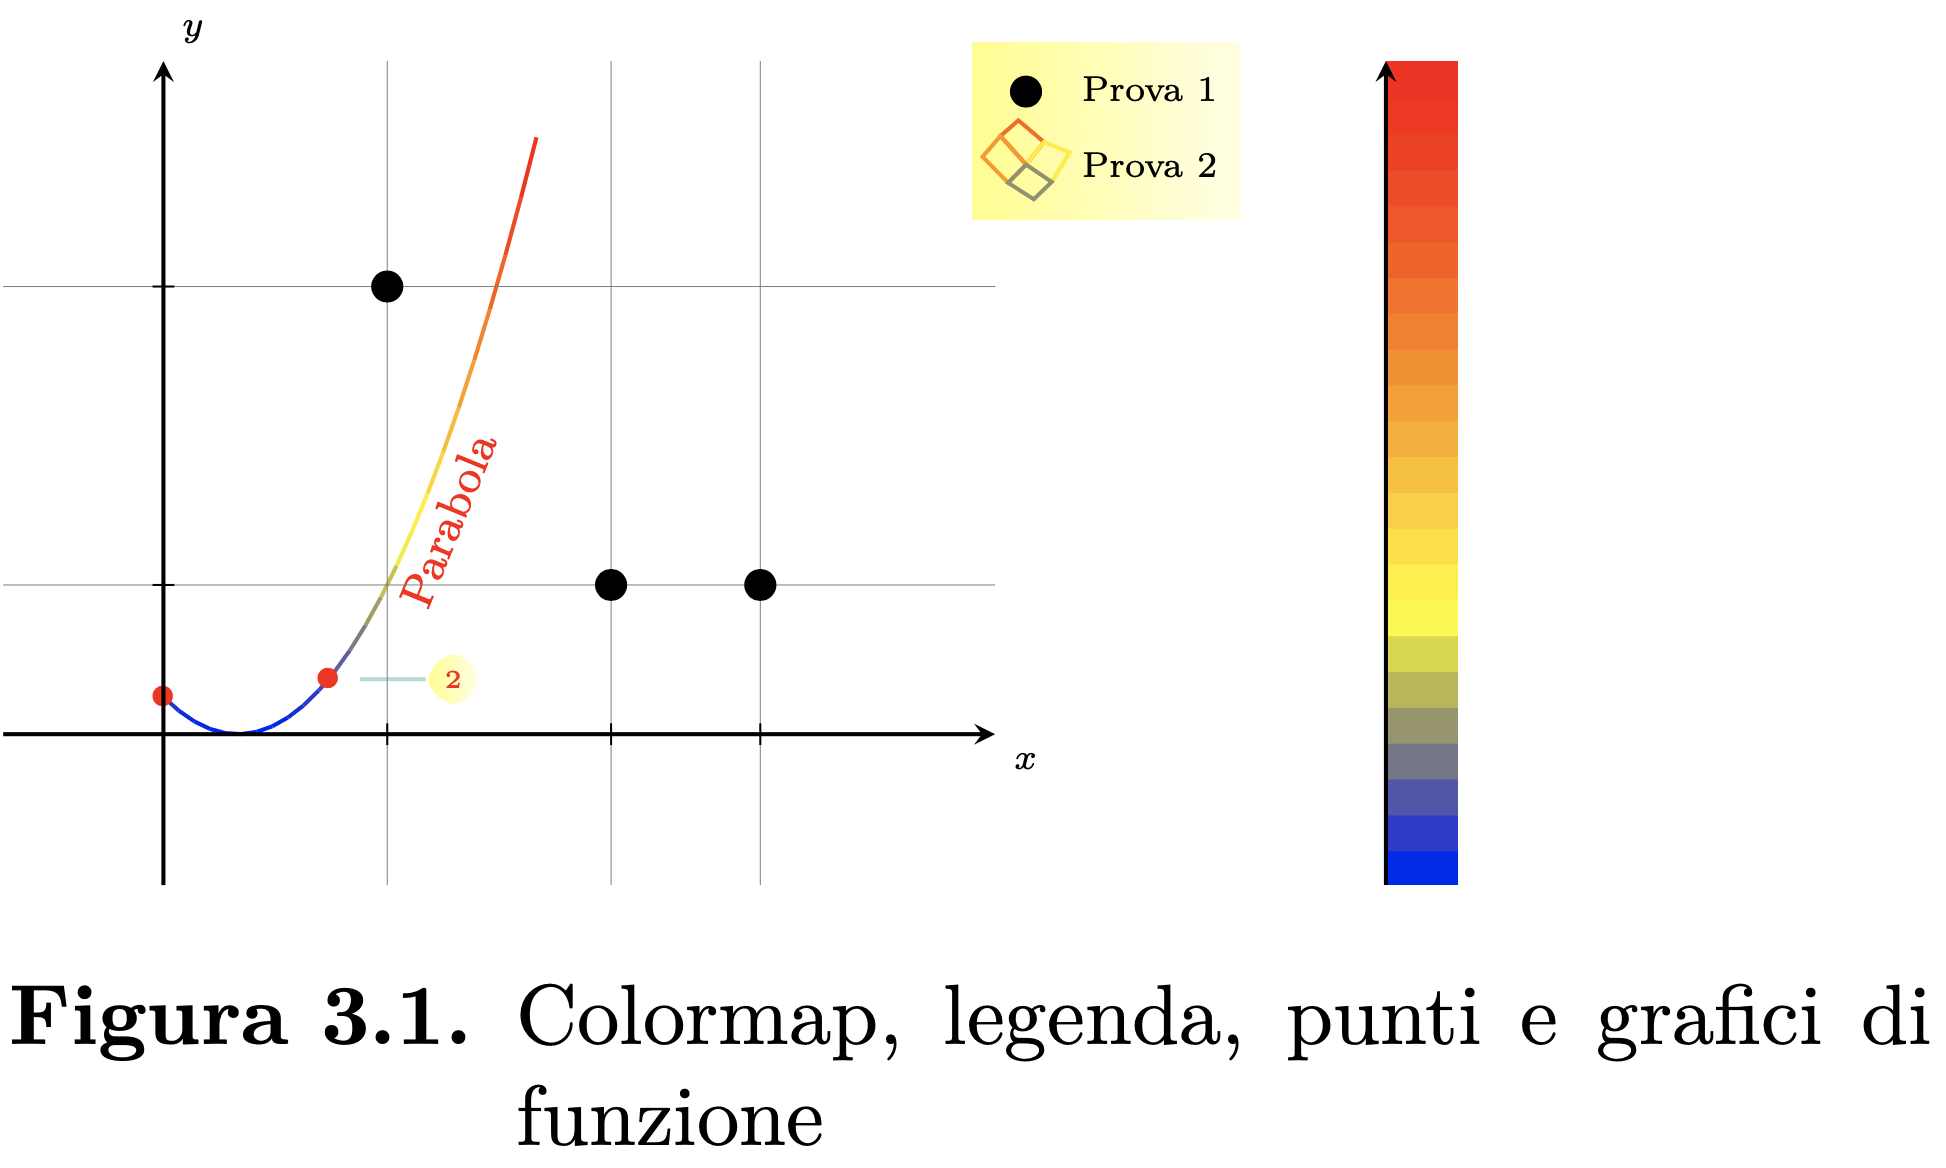
\includegraphics[scale=.4]{FileAusiliari/Screenshots/Figura3-1.png}
\end{figure}

\newpage

\begin{verbatim}
\begin{figure}[ht]\centering
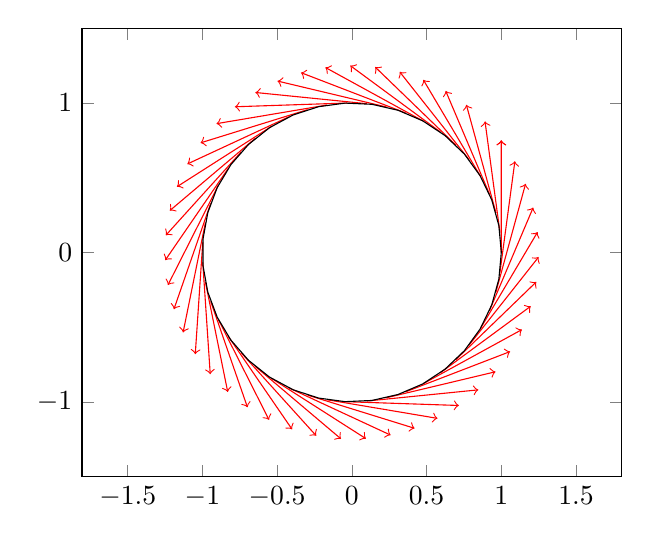
\begin{tikzpicture} \begin{axis}[
    axis equal, xmin=-1.5, xmax=1.5, ymin=-1.5, ymax=1.5]
    \addplot [samples=48, domain=0:2*pi,->,blue, variable=\t,
        quiver={
            u={-sin(deg(t))},
            v={cos(deg(t))},
            scale arrows=0.75,
            colored=red},] ({cos(deg(t))}, {sin(deg(t))});
    \addplot [samples=36, domain=0:2*pi] ( {cos(deg(x))}, {sin(deg(x))} );
\end{axis}
\end{tikzpicture}
\caption{Parametrizzazioni}
\end{figure}
\end{verbatim}

\begin{figure}[ht]\centering
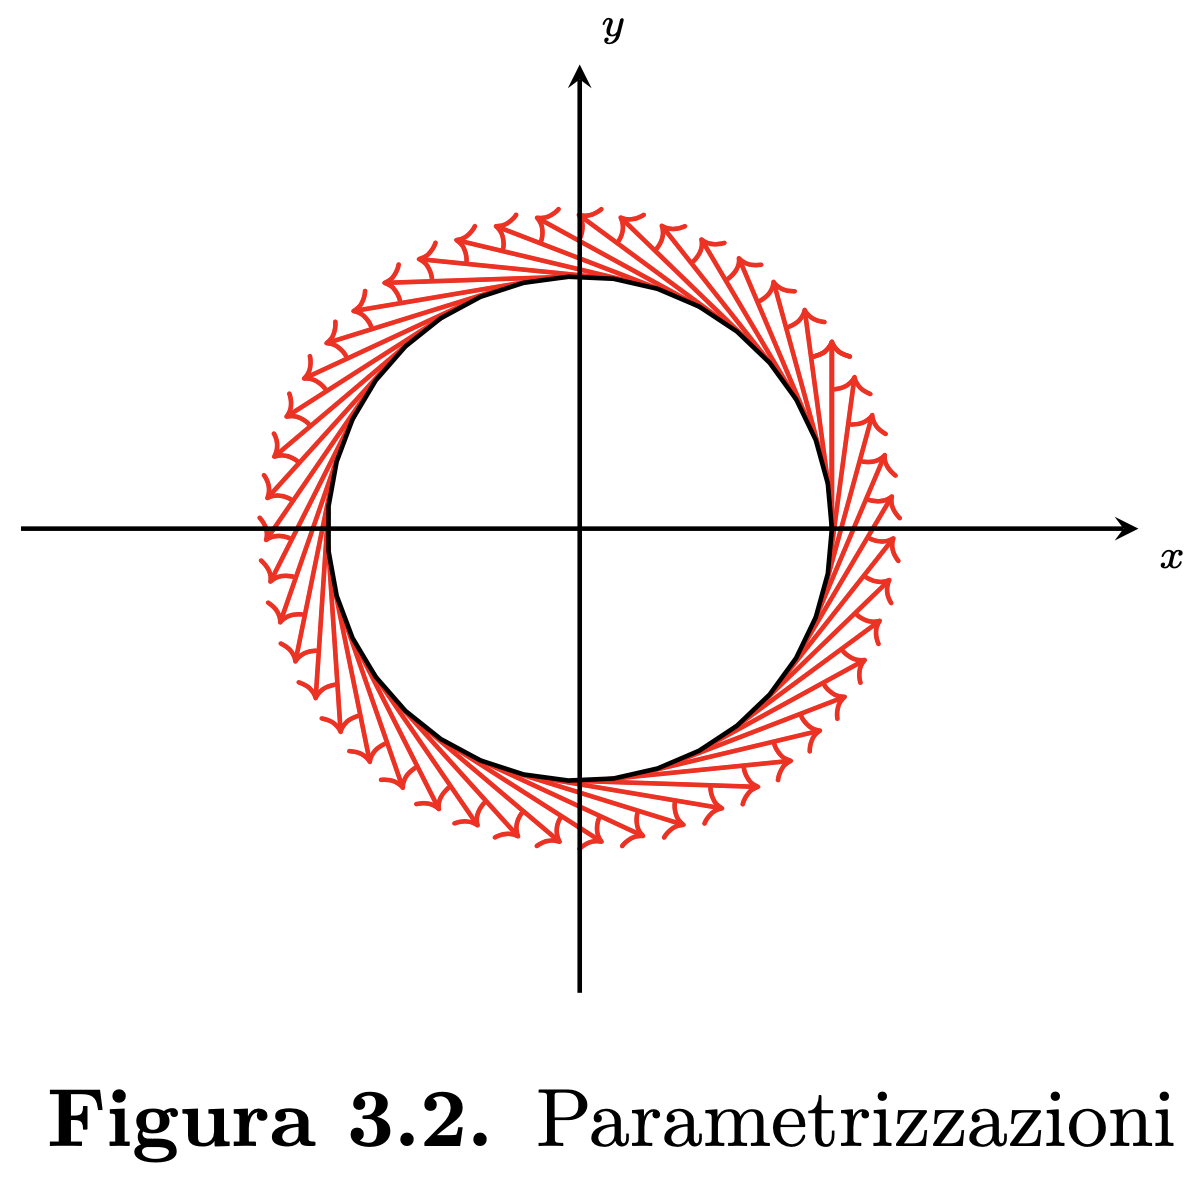
\includegraphics[scale=.4]{FileAusiliari/Screenshots/Figura3-2.png}
\end{figure}

\newpage

\begin{verbatim}
\begin{figure}[ht]\centering
\begin{tikzpicture}
\begin{axis}[xmin=-5, xmax=5, ymin=-28, axis equal]
\addplot [samples=24, domain=0:2*pi, dashed, data cs=polar,
	top color=Blues-I, bottom color=Blues-B] (deg(x),30);
\addplot [name path=Y, samples=24, domain=0:2*pi, dashed,
    data cs=polar] (deg(x),30);
\addplot [GnBu-M, name path=X, domain=0:360, samples=36,
    smooth, data cs=polar](x, {30-8*sin(3*x)});
\addplot[green] fill between[of=Y and X];
\addplot [samples=36,domain=0:30, dashed,
    data cs=cart] {.025*x^2} node [pos=1] {Nodo};
\addplot [mark=oplus, only marks] coordinates {(0,0)};
\node[pin=120:{Pin nodo}] at (0,0) {};
\end{axis}
\end{tikzpicture}
\caption{Filling, nodi e pin}
\end{figure}	
\end{verbatim}

\begin{figure}[ht]\centering
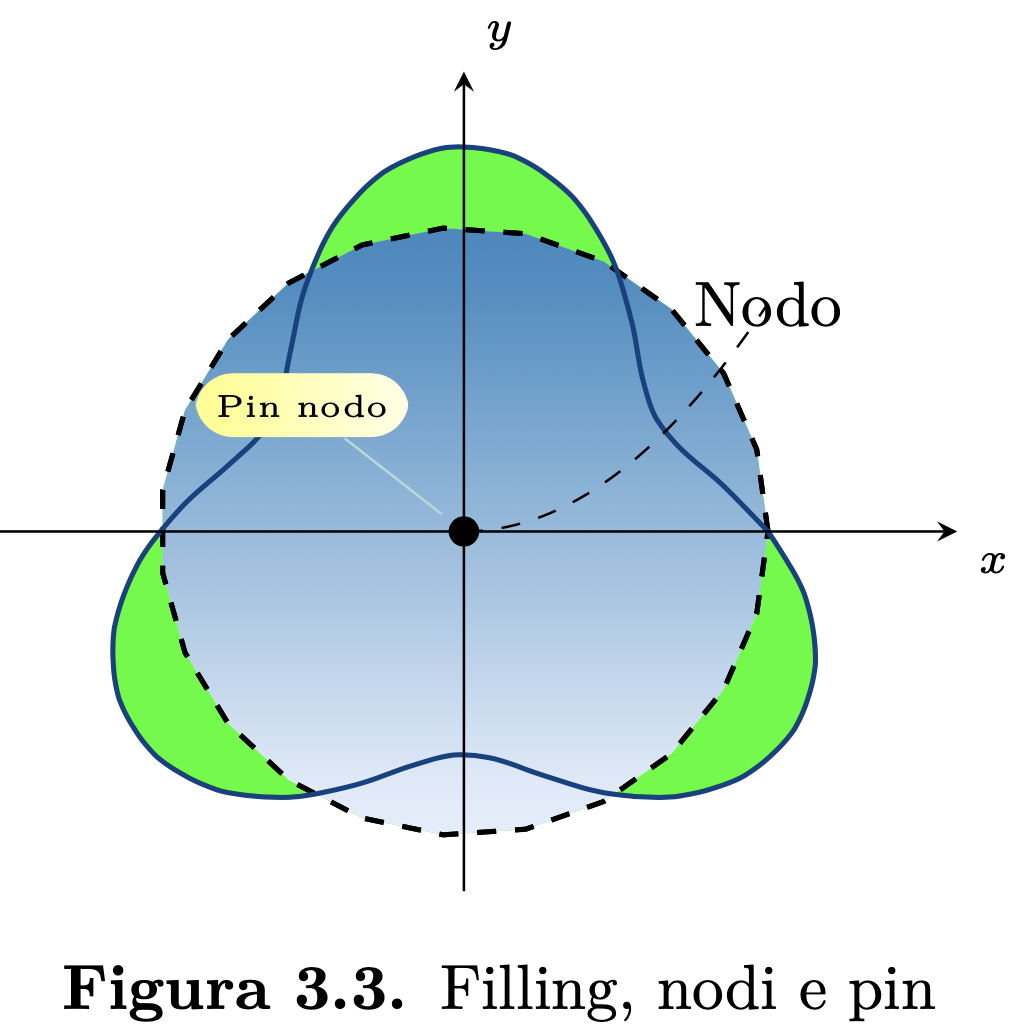
\includegraphics[scale=.5]{FileAusiliari/Screenshots/Figura3-3.png}
\end{figure}

\newpage
\begin{verbatim}
\begin{figure}[ht]\centering
\begin{tikzpicture}[scale=.8]
\begin{axis}[axis equal=false, xmin=-1, xmax=2, ymin=-3.5, ymax=1]
\addplot[red, patch type sampling, patch type= cubic spline, domain=0:2, smooth]{ln(x)};
\draw (0,0) .. controls (1,-1.2) and (1,1) .. (2,1);
   \end{axis}
\end{tikzpicture}
\caption{Interpolazione, paths}
\end{figure}
\end{verbatim}

\begin{figure}[ht]\centering
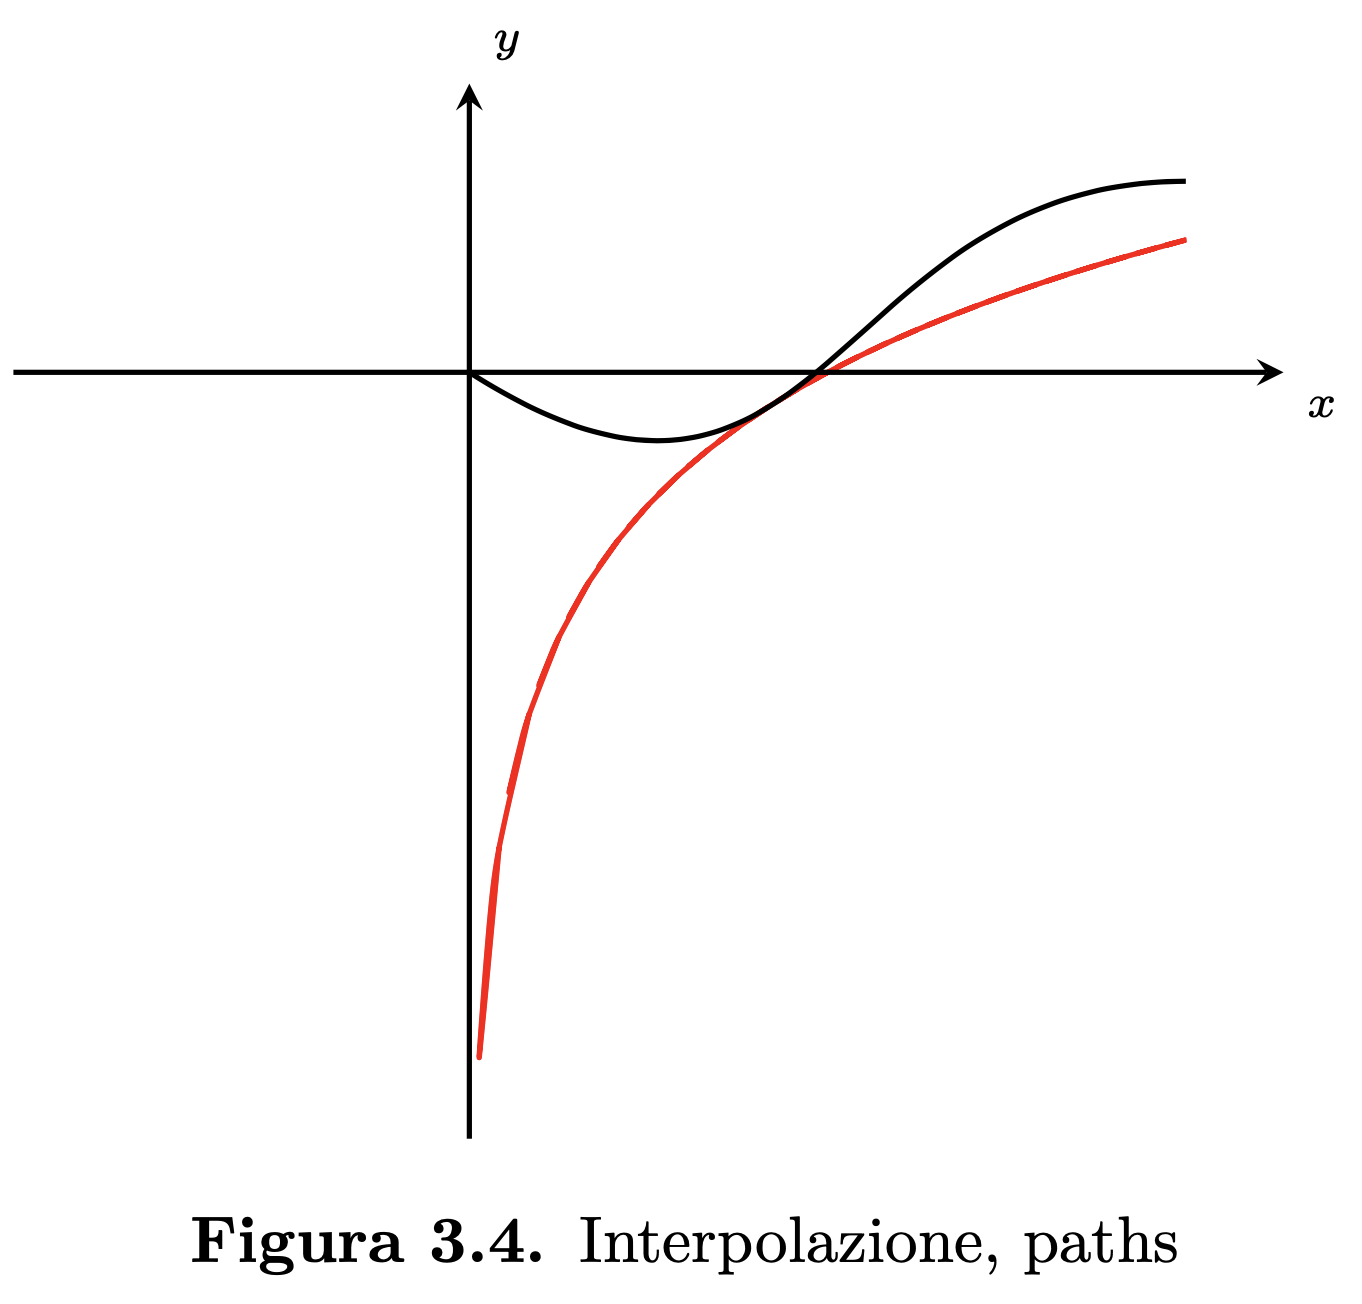
\includegraphics[scale=.5]{FileAusiliari/Screenshots/Figura3-4.png}
\end{figure}

\newpage

\begin{verbatim}
\begin{figure}[ht]\centering
\begin{tikzpicture}
\begin{axis}[
    colormap/PuBu,
    samples=12, domain=-5:5, y domain=-4:4,  xmin=-5, xmax=5, ymin=-4, ymax=4]
    \addplot3 [surf,     samples=24,    samples y=40] {x^2+y^2-1};
\end{axis}
\end{tikzpicture}	
\caption{Superfici 3D}
\end{figure}
\end{verbatim}

\begin{figure}[ht]\centering
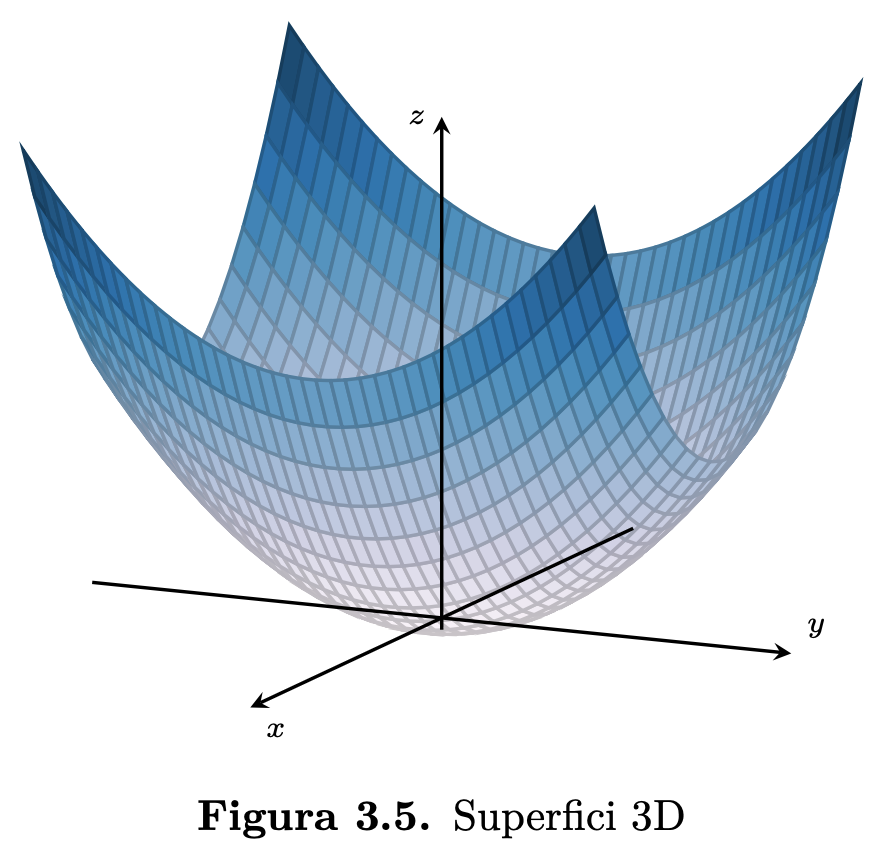
\includegraphics[scale=.6]{FileAusiliari/Screenshots/Figura3-5.png}
\end{figure}

\newpage

\begin{verbatim}
\begin{figure}[ht]\centering
\begin{tikzpicture}[spy using outlines={}]
\begin{axis}[axis equal=false, grid=major, xmin=-1, xmax=6, ymin=0, ymax=1,
every axis plot post/.append style={thick}, xtick=data, ytick=data]
\addplot[line join=round, green] coordinates {(1, 0) (1,.75) (3, 0.9) (4, .75) (5, 0.8)};
\addplot[line join=bevel, blue] coordinates {(0, 0) (1, 0.4) (3, 0.2) (4, 1) (5, 0.9)};
\coordinate (spypoint)     at (1,.4);
\coordinate (magnifyglass) at (-2,.25);
\end{axis}
\spy [blue, size=1.5cm, circle, magnification=5, connect spies] on (spypoint) in
                                 node[fill=white] at (magnifyglass);
\end{tikzpicture}	
\caption{Ambiente spy}
\end{figure}
\end{verbatim}

\begin{figure}[ht]\centering
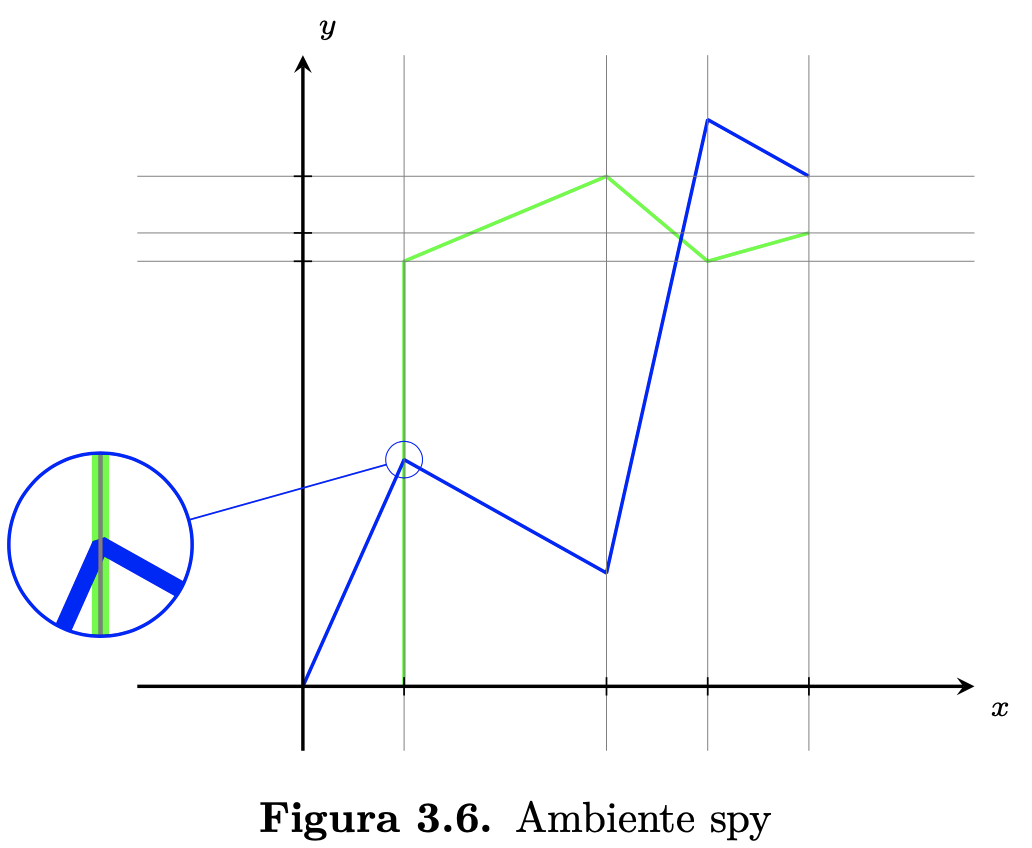
\includegraphics[scale=.5]{FileAusiliari/Screenshots/Figura3-6.png}
\end{figure}

\newpage
\begin{verbatim}
\begin{figure}[ht]\centering
\begin{tikzpicture}[scale=.75]
	\begin{axis}[xmin=0, xmax=3.5, ymin=0, ymax=5]
	\draw [name path=ellipse] (2,3) ellipse (1.5 and 1.25);
	\draw [name path=rectangle] (1.5,1.5) rectangle (3,5);
	\fill [red, opacity=0.5, name intersections={of=ellipse and rectangle}]   
		(intersection-1) circle (2pt) node[above right] {1}
        (intersection-2) circle (2pt) node[above left] {2} 
        (intersection-3) circle (2pt) node[below left] {3} 
        (intersection-4) circle (2pt) node[below right] {4};
	\end{axis}
\end{tikzpicture}
\caption{Intersezione di figure}
\end{figure}
\end{verbatim}

\begin{figure}[ht]\centering
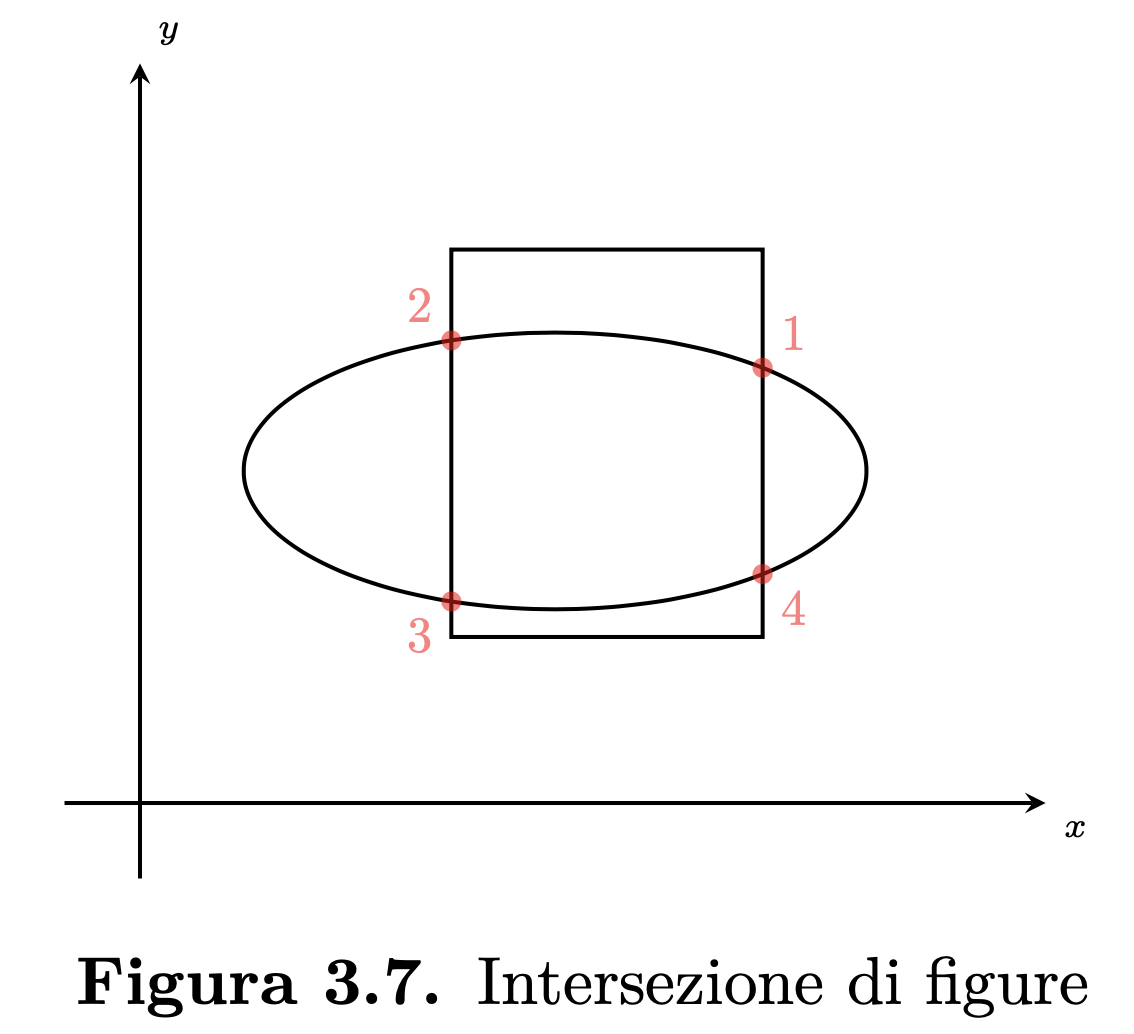
\includegraphics[scale=.5]{FileAusiliari/Screenshots/Figura3-7.png}
\end{figure}

\newpage
\begin{verbatim}
\begin{figure}[ht]\centering
\tdplotsetmaincoords{70}{135}
\begin{tikzpicture}[scale=3,
tdplot_main_coords]
\tdplotsphericalsurfaceplot[parametricfill]{36}{36}
{sqrt(15/2)*sin(\tdplottheta)*cos(\tdplottheta)}{black!10}{\tdplotphi}
    {\draw[color=black,thick,->] (0,0,0) -- (2,0,0) node[anchor=north east]{$x$};}
    {\draw[color=black,thick,->] (0,0,0) -- (0,2,0) node[anchor=north west]{$y$};}
    {\draw[color=black,thick,->] (0,0,0) -- (0,0,2) node[anchor=south]{$z$};}
\end{tikzpicture}
\caption{Tikz-3dplot - Esempio 1}
\end{figure}
\end{verbatim}

\begin{figure}[ht]\centering
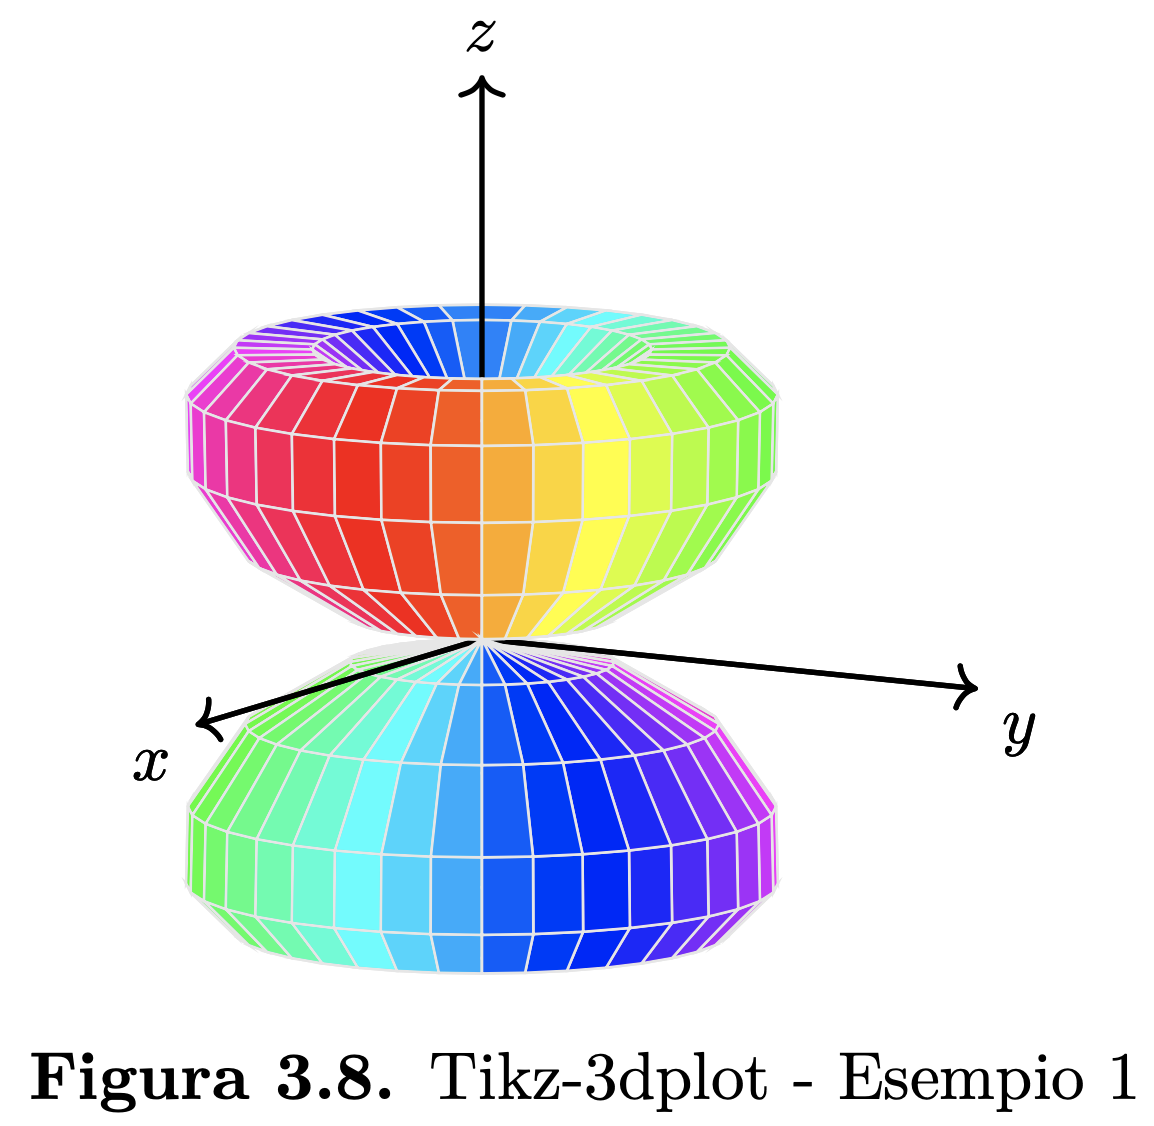
\includegraphics[scale=.6]{FileAusiliari/Screenshots/Figura3-8.png}
\end{figure}

\newpage
\begin{verbatim}
\begin{figure}[ht]\centering
\tdplotsetmaincoords{60}{110}
\begin{tikzpicture}[scale=5,tdplot_main_coords]
\pgfmathsetmacro{\rvec}{.8}
\pgfmathsetmacro{\thetavec}{30}
\pgfmathsetmacro{\phivec}{60}
    \coordinate (O) at (0,0,0);
    \draw[thick,->] (0,0,0) -- (1,0,0) node[anchor=north east]{$x$};
    \draw[thick,->] (0,0,0) -- (0,1,0) node[anchor=north west]{$y$};
   \draw[thick,->] (0,0,0) -- (0,0,1) node[anchor=south]{$z$};
    \tdplotsetcoord{P}{\rvec}{\thetavec}{\phivec}
    \draw[-stealth,color=red] (O) -- (P);
    \draw[dashed, color=red] (O) -- (Pxy);
    \draw[dashed, color=red] (P) -- (Pxy);
    \tdplotdrawarc{(O)}{0.2}{0}{\phivec}{anchor=north}{$\phi$}
    \tdplotsetthetaplanecoords{\phivec}
    \tdplotdrawarc[tdplot_rotated_coords]{(0,0,0)}{0.5}{0}%
        {\thetavec}{anchor=south west}{$\theta$}
    \draw[dashed,tdplot_rotated_coords] (\rvec,0,0) arc (0:90:\rvec);
    \draw[dashed] (\rvec,0,0) arc (0:90:\rvec);
    \tdplotsetrotatedcoords{\phivec}{\thetavec}{0}
    \tdplotsetrotatedcoordsorigin{(P)}
    \draw[thick,tdplot_rotated_coords,->] (0,0,0)
        -- (.5,0,0) node[anchor=north west]{$x’$};
    \draw[thick,tdplot_rotated_coords,->] (0,0,0)
        -- (0,.5,0) node[anchor=west]{$y’$};
    \draw[thick,tdplot_rotated_coords,->] (0,0,0)
        -- (0,0,.5) node[anchor=south]{$z’$};
    \draw[-stealth,color=blue,tdplot_rotated_coords] (0,0,0) -- (.2,.2,.2);
    \draw[dashed,color=blue,tdplot_rotated_coords] (0,0,0) -- (.2,.2,0);
    \draw[dashed,color=blue,tdplot_rotated_coords] (.2,.2,0) -- (.2,.2,.2);
    \tdplotdrawarc[tdplot_rotated_coords,color=blue]{(0,0,0)}{0.2}{0}%
        {45}{anchor=north west,color=black}{$\phi’$}
    \tdplotsetrotatedthetaplanecoords{45}
    \tdplotdrawarc[tdplot_rotated_coords,color=blue]{(0,0,0)}{0.2}{0}%
        {55}{anchor=south west,color=black}{$\theta’$}
\end{tikzpicture}
\caption{Tikz-3dplot - Esempio 2}
\end{figure}
\end{verbatim}

\begin{figure}[ht]\centering
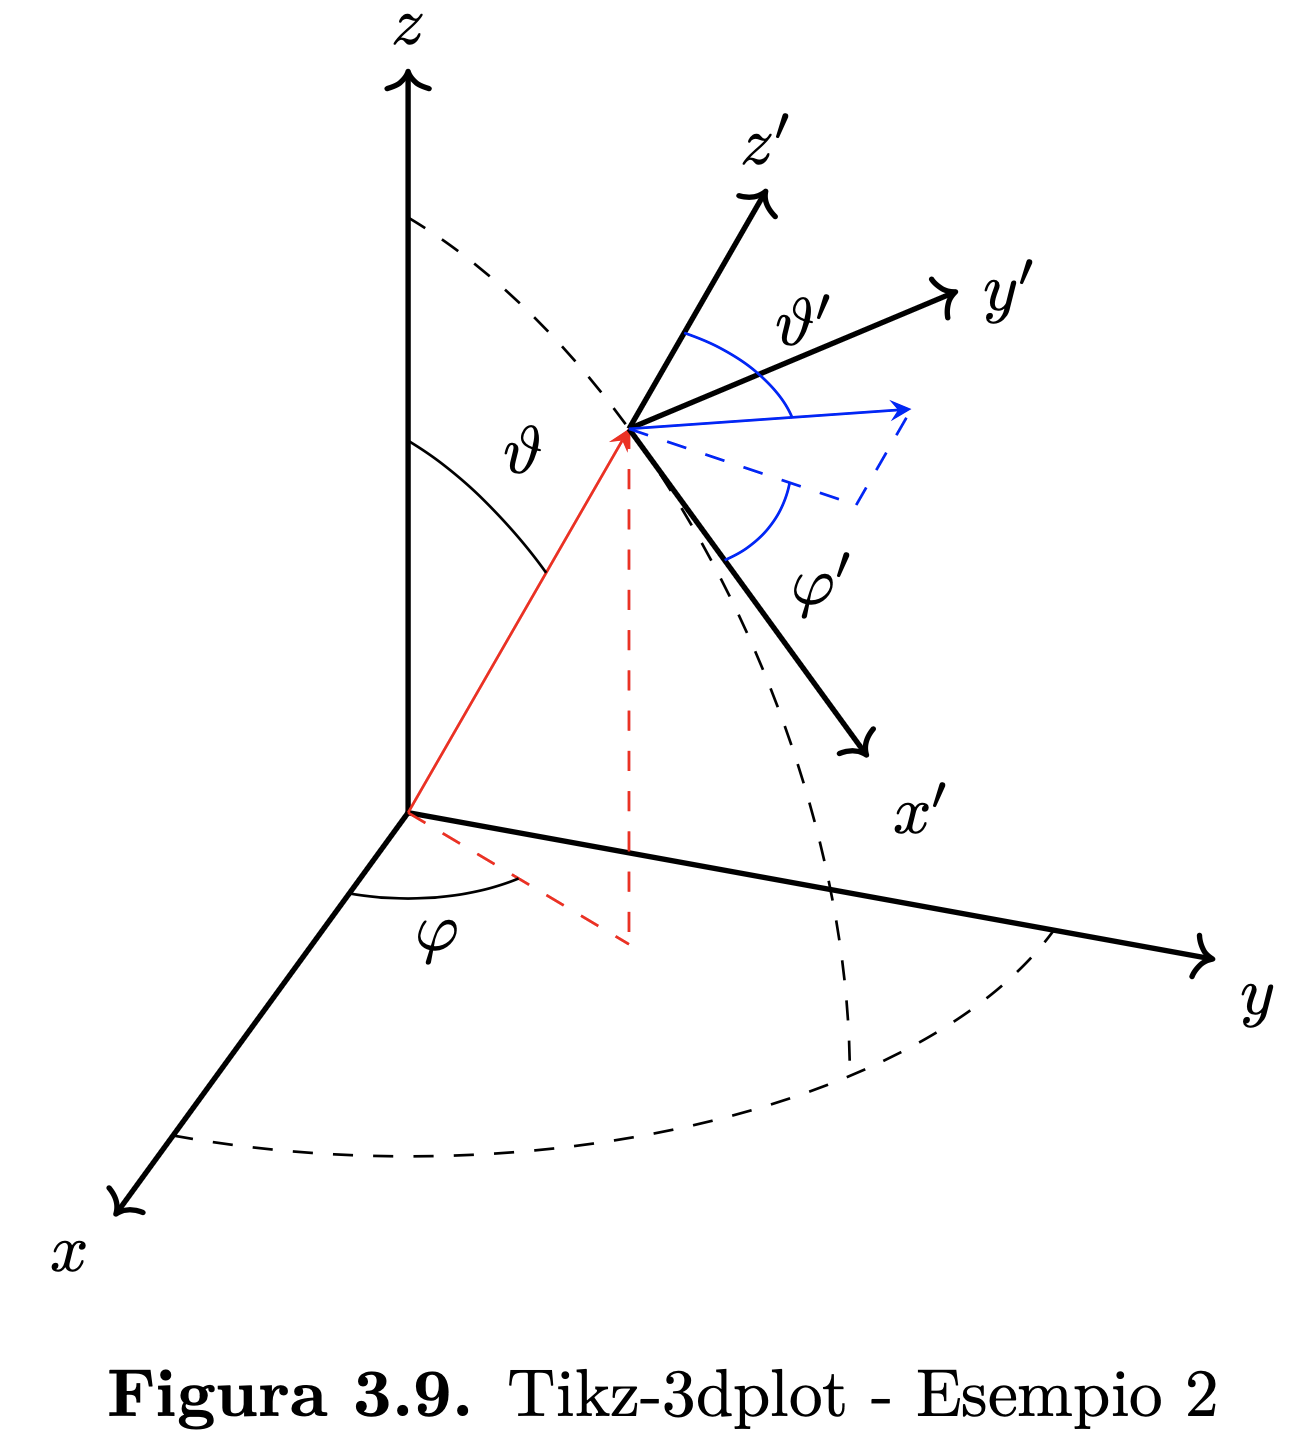
\includegraphics[scale=.25]{FileAusiliari/Screenshots/Figura3-9.png}
\end{figure}